
% \subsection{水治理变化的驱动力分析}\label{ch4:sec:mechanism}

\begin{figure}[th!]
	\centering
	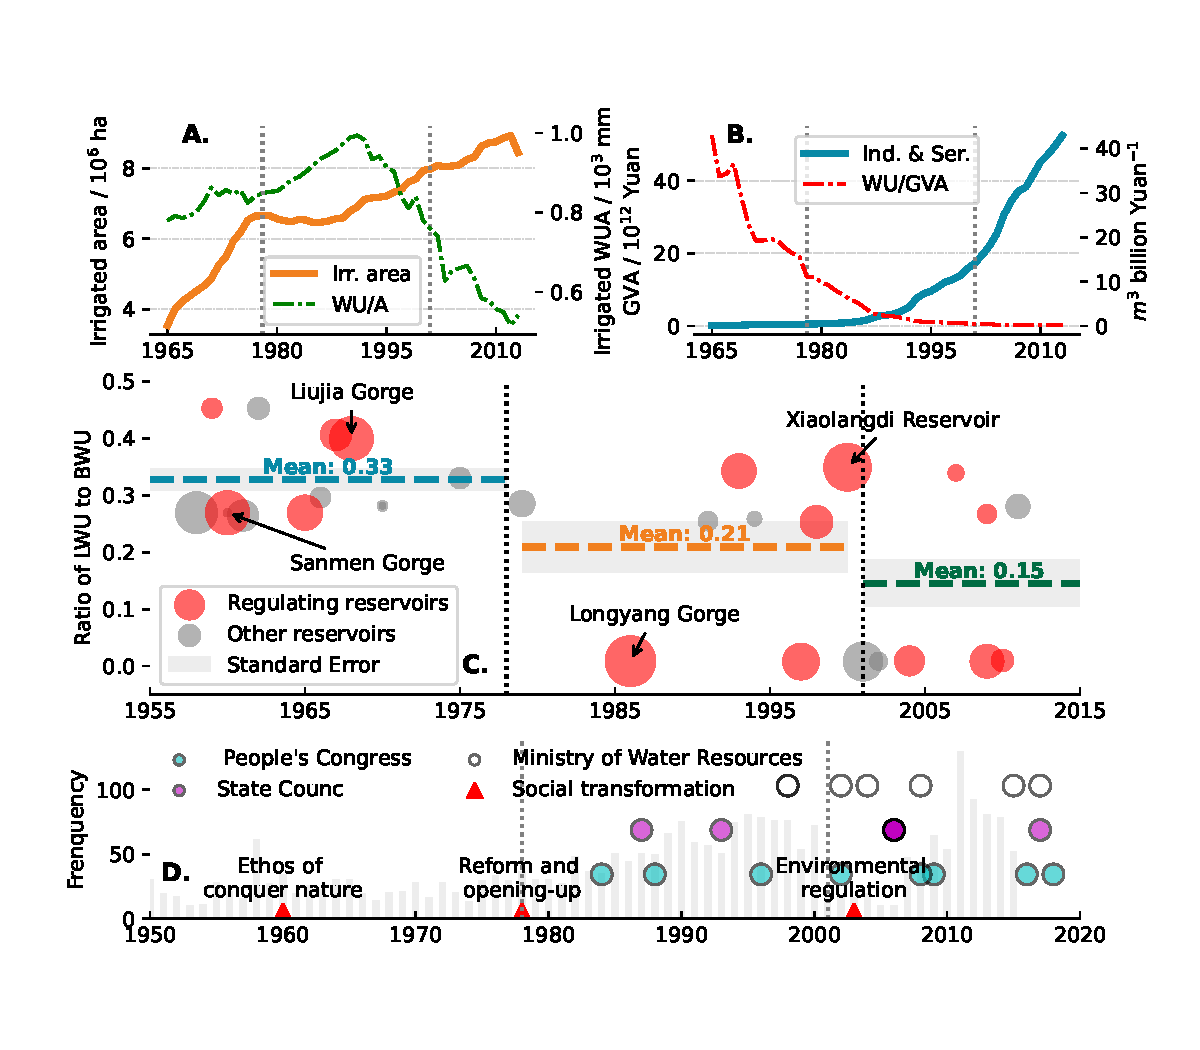
\includegraphics[width=\textwidth]{img/ch4/causes.pdf}
	\caption[黄河流域水治理体制变化的驱动因素]{
		黄河流域水治理体制变化的驱动因素。
		\textbf{A.}总灌溉面积($A$, 橙色线)和用水强度($WU/A$,用水量除以灌溉面积,绿点线)的变化。
        \textbf{B.}工业和服务业的总增加值(蓝线,$GVA$)变化及其用水强度($WU/GVA$,WU除以GVA,红点线)。
        \textbf{C.}每个水库的完工时间及其所在区域的用水量(Local Water Use, LWU)占水库完工时流域总用水量(Basinal Water Use, BWU)的百分比。红圈为负责黄河流域综合调度的水库。每个圆圈的大小表示其储水能力的大小。
        \textbf{D.}社会转型(红色三角形)和国家层面的治理政策(圆圈,不同颜色表示由不同的国家机构签署,越靠上代表国家机构的登记越高,详见表\ref{ch4:tab:policies})。浅灰色条形图以流域尺度(黄河大事件)计算与黄河流域有关的官方治理文献记录。}\label{ch4:fig:mechanism}
\end{figure}


\begin{figure}[tb]
    \centering
    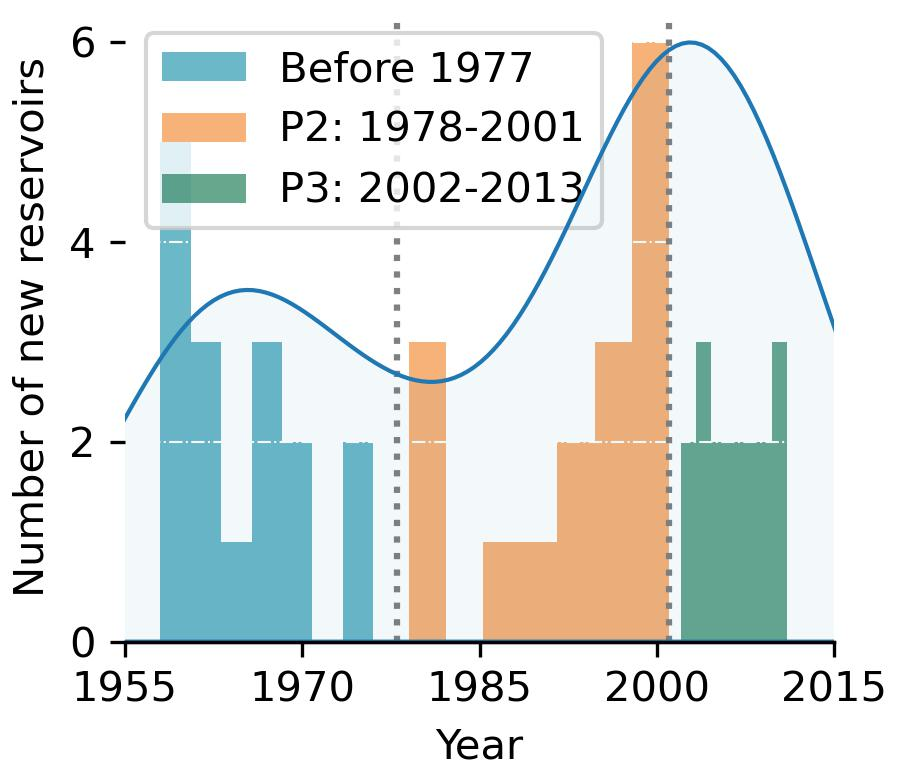
\includegraphics[width=0.6\linewidth]{img/ch4/reservoirs.jpg}
    \caption{黄河流域各年新增水库数量}\label{ch4:fig:reservoirs}
\end{figure}


本节进一步探讨了致使IWGI变化的原因,灌溉区扩张和工业和服务业的经济增长是推动“集中供水时期”和“治理转型时期”两个阶段变化的关键。
黄河流域的用水需求在“集中供水时期”迅速增加,尤其是灌溉农业面积以$0.25*10^6 ha/yr$的速度迅速扩张(图\ref{ch4:fig:mechanism}~A),同时通过建设水库增加供应(图~\ref{ch4:fig:reservoirs})。
进入“治理转型时期”后,尽管灌溉区扩张停滞,但工业和服务业的发展开始增长,共同推动流域用水需求的进一步增加(图\ref{ch4:fig:mechanism}~A和B)。
接下来从“治理转型时期”到“适应增强时期”的演变过程中,水分利用效率变化最明显。
在“适应增强时期”,不仅工业和城市服务也承担了更重要的经济角色(由总增加值GVA表示,图\ref{ch4:fig:mechanism}~B),灌溉面积也恢复了缓慢扩张(图\ref{ch4:fig:mechanism}~A)。
但因用水效率的普遍提高,单位灌溉面积或单位产量的用水量都显著下降(图~\ref{ch4:fig:mechanism}~A和图~\ref{ch4:fig:mechanism}~B),因此部门和地区之间的用水差异在不断缩小,但流域水资源压力总体、持续维持在较高水平,公平合理分配宝贵水资源的压力越来越大(图~\ref{ch4:fig:IWGI}~A)。

最后,环境背景、社会文化、水治理政策等因素为三个时期的指标变化都产生了影响。
我们首先计算了每个水库的区域用水量和流域用水量之比,较高的比值代表了该水库等潜在作用更有可能是旨在为该流域供水而不是流域调度;此外,流域调度的枢纽水库也以红色进行了标记(图~\ref{ch4:fig:mechanism}~C)。
可以看到,在阶段一的“集中供水时期”,受“征服自然”的社会口号引领,大部分水库都建在需水量较大的地区,因此区域用水量和流域用水量之比值明显较高($p<0.01$,见图~\ref{ch4:fig:mechanism}~C)。
进入“治理转型时期”之后,新建水库的数量明显减少且多为枢纽水库,但全流域层次的法律法规(包括著名的“八七”分水方案)开始被不断提出,流域内的治理记录也迅速增加,可见此时期层出不穷的流域政策已深刻影响了流域水治理,流域水治理正在进行一场从工程措施向非工程措施的“治理转型”(图~\ref{ch4:fig:mechanism}~D, $p<0.01$和图\ref{ch4:fig:reservoirs})。
最后在“适应增强时期”,持续高位的水压力已成为制约区域发展的瓶颈,亟需通过节水转型和跨区域协调、调水来满足经济发展的用水需求,因此并且“大规模进行环境治理和节水转型”的国家战略指导下,有关部门提出了更多的、级别更高的水治理决策(图~\ref{ch4:fig:mechanism}~D)。
综上所述,从“集中供水时期”到“治理转型时期”的转变与当时水资源供需的增加相一致;而“治理转型时期”到“适应增强时期”的演变过程则是在水资源压力趋于稳定的同时,由社会监管政策和节水转型带来的效率提高所驱动的。